\documentclass[a4,compress]{beamer}

%!TeX spellcheck = en-GB

% chktex-file 18

\usepackage{beamerthemesplit}

\usepackage{amsmath, amsfonts, amssymb}
\usepackage{amsthm}
\usepackage{mathtools}
\usepackage{physics}

\usepackage{graphicx}
\graphicspath{{../Manuscript/Title/img/} {../External_plots/} {../Output/} {../Statistics/}}

\usepackage[utf8]{inputenc}

\usepackage{times}
\usepackage[T1]{fontenc}

\usepackage[english]{isodate}

\newcommand{\ee}{\operatorname{e}}          % Euler's number
\newcommand{\ii}{\mathrm{i}}                % imaginary unit
\newcommand{\ad}[1]{a_{#1}^{\dagger}}       % creation operator
\newcommand*\mean[1]{\overline{#1}}         % mean

\mode<presentation>
{
  \usetheme{Warsaw}
  \setbeamercovered{transparent}
}

\AtBeginSection[]
{
  \begin{frame}
    \frametitle{Outline}
    \tableofcontents[currentsection]
  \end{frame}
}

\addtobeamertemplate{navigation symbols}{}{%
    \usebeamerfont{footline}%
    \usebeamercolor[fg]{footline}%
    \hspace{1em}%
    \insertframenumber/\inserttotalframenumber
}

\addtobeamertemplate{title page}{
\includegraphics[width=1.3cm]{unibuc} \hfill 
\includegraphics[width=1.6cm]{fizica}}{}

\title[Fingerprints of classical structures in quantum chaos]{Fingerprints of classical phase space structure in quantum chaos}
\subtitle{Bachelor Thesis}

\author{
  Sebastian MICLUȚA-CÂMPEANU \\
  \hspace{6cm} {\small	Scientific Advisers:} \\
  \hspace{6.35cm} {\small Prof.~dr.~Virgil BĂRAN} \\
  \hspace{6.35cm} {\small Lect.~dr.~Roxana ZUS}
}

\institute[Universitatea din București]
{
  Universitatea din București \\
  Facultatea de Fizică
}
\date{\small Bucharest, 29 \printdayoff\today}

\begin{document}

%%%%%%%%%%%%%%%%%%%% slide 1 %%%%%%%%%%%%%%%%%%%%%%%%%%%%%%%%%%%%%%

\begin{frame}[plain]
 \titlepage
\end{frame}


%%%%%%%%%%%%%%%%%%%% slide 2 %%%%%%%%%%%%%%%%%%%%%%%%%%%%%%%%%%%%%%

\begin{frame}{Outline}
  \tableofcontents[]%pausesections]
\end{frame}

\section[Intro]{Introduction}

%%%%%%%%%%%%%%%%%%%% slide 3 %%%%%%%%%%%%%%%%%%%%%%%%%%%%%%%%%%%%

\begin{frame}
  \begin{itemize}
    \item The aim of this thesis is to study the correspondence
    between the classical chaotic behaviour of nuclear surface vibrations
    and the quantum features of energy spectra of same system.
  \end{itemize}
\end{frame}

\section[Chaos]{Chaotic dynamics}

\subsection{Classical Chaos}

%%%%%%%%%%%%%%%%%%%% slide 4 %%%%%%%%%%%%%%%%%%%%%%%%%%%%%%%%%%%%

% \subsection{Fundamental notions}

\begin{frame}
  \begin{itemize}
    \item Hamilton's equations
    \begin{align*}
      \dot{q_k} = \pdv{\mathcal{H}}{p_k}, &&
      \dot{p_k} = -\pdv{\mathcal{H}}{q_k}
    \end{align*}
    \item Action-angle variables
    \begin{align*}
      I_k = \frac{1}{2\pi}\oint p_k \dd{q_k}, &&
      \theta_k = \omega_k(I_k) \Delta t
    \end{align*}
    \item Integrability: A system is \emph{integrable} if the number of degrees
    of freedom is equal to the number of constants of the motion
    (in involution which each other).
    \item For integrable systems with $n$ degrees of freedom, the trajectory
    in phase space is constrained to a $n$-torus.
  \end{itemize}
\end{frame}

%%%%%%%%%%%%%%%%%%%% slide 5 %%%%%%%%%%%%%%%%%%%%%%%%%%%%%%%%%%%%

\begin{frame}{K.A.M. Theorem}
  \begin{itemize}
    \item If the motion of a system described by an integrable
    Hamiltonian is perturbed with a small non-integrable term and
    the frequencies (\(\omega_k = \dot{\theta}_k\)) of the unperturbed motion
    are such that for \(k=1,\dotsc,n\), we have
    \(m_k\, \omega_k \neq 0, \forall\ m_k \in \mathbb{Z}\),
    then the motion will remain on the $n$-torus, except for a small
    set of initial conditions, for which the trajectories escape on the
    energy hyper-surface.

  \end{itemize}
\end{frame}

%%%%%%%%%%%%%%%%%%%% slide 6 %%%%%%%%%%%%%%%%%%%%%%%%%%%%%%%%%%%%

\begin{frame}{Indicators of chaos}
  \begin{columns}[c]
  \begin{column}{0.6\textwidth}
    \begin{itemize}
      \item Poincaré sections: Slices of the phase space which reduce the
      dimensionality by one.
      \item Liapunov exponent
      \[
        \lambda = \lim\limits_{t \to \infty} \frac{1}{t} \ln{\frac{\dd{x}(t)}{\dd{x}(0)}}
      \]
      \item Chaos is characterised by sensitivity to the initial conditions
      (\(\lambda > 0\)).
    \end{itemize}
  \end{column}
  \begin{column}{0.4\textwidth}
    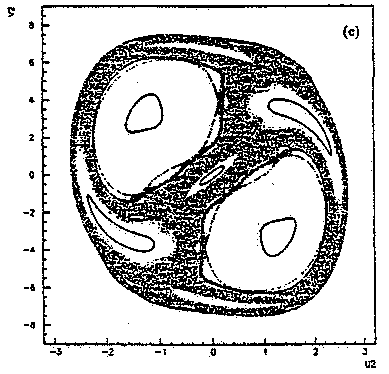
\includegraphics[width=0.9\textwidth]{ponicare-sections-e_120}
  \end{column}
  \end{columns}

\end{frame}

\subsection{Quantum Chaos}

%%%%%%%%%%%%%%%%%%%% slide 7 %%%%%%%%%%%%%%%%%%%%%%%%%%%%%%%%%%%%

\begin{frame}
  \begin{itemize}
    \item In Quantum Mechanics we can no longer speak of trajectories
    or sensitivity to the initial conditions.
    \item We need a way to compare spectra from different systems
    in order to search for common patterns or features.
    \item We can use the level spacings (\(E_{n+1} - E_n\)) to build
    the nearest neighbour level spacing distributions.
  \end{itemize}
\end{frame}

%%%%%%%%%%%%%%%%%%%% slide 8 %%%%%%%%%%%%%%%%%%%%%%%%%%%%%%%%%%%%

\begin{frame}{Giving meaning to quantum chaos}
  \begin{itemize}
    \item Berry-Tabor conjecture: The quantum counterpart of a classically integrable
    system has a Poissonian nearest neighbour distribution.
    \[
      P_P(s) = \ee^{-s}
    \]
    \item Bohigas-Gianoni-Schmit conjecture: The nearest neighbour distribution
    of a quantum system with a classically chaotic counterpart is given by
    the Wigner distribution.
    \[
      P_W(s) = \frac{\pi}{2} s \exp(-\frac{\pi}{4} s^2)
    \]
  \end{itemize}
\end{frame}

%%%%%%%%%%%%%%%%%%%% slide 9 %%%%%%%%%%%%%%%%%%%%%%%%%%%%%%%%%%%%

\begin{frame}{Other measures}
  \begin{itemize}
    \item Cumulative spacing distribution
    \[
      I(s) = \int_0^s P(x) \dd{x}
    \]
  \end{itemize}
\end{frame}

\section[Model]{Surface vibrations}

%%%%%%%%%%%%%%%%%%%% slide 10 %%%%%%%%%%%%%%%%%%%%%%%%%%%%%%%%%%%%

\begin{frame}
  \begin{itemize}
    \item The radius of the nuclear surface
    \[
      R(\theta, \varphi) = R_0 \left( 1 + \sum_{\lambda, \mu}
          \alpha_{\lambda,\mu}^* Y_{\lambda,\mu}(\theta, \varphi) \right)
    \]
    \item For \(\lambda = 2\) we describe the surface in terms of
    quadrupole vibrations.
    \item \(\alpha_{\lambda,\mu}\) become dynamical degrees of freedom
  \end{itemize}
\end{frame}

%%%%%%%%%%%%%%%%%%%% slide 11 %%%%%%%%%%%%%%%%%%%%%%%%%%%%%%%%%%%%

\begin{frame}
  \begin{itemize}
    \item We want to study only the vibrations of the surface, so we will
    use the intrinsic reference frame of the nucleus. Thus we will only have
    2 degrees of freedom.
    \item The Hamiltonian of the system will be given by
    \[
    \begin{split}
      \mathcal{H}(q_0,p_0,q_2,p_2) &= \frac{A}{2}(p_0^2 + p_2^2 + q_0^2 + q_2^2) \\
      &+ \frac{B}{\sqrt{2}}q_0(3q_2^2 - q_0^2)
      + \frac{D}{4}{(q_0^2 + q_2^2)}^2
    \end{split}
    \]
  \end{itemize}
\end{frame}

%%%%%%%%%%%%%%%%%%%% slide 12 %%%%%%%%%%%%%%%%%%%%%%%%%%%%%%%%%%%%

\begin{frame}
  \begin{itemize}
    \item Quantised Hamiltonian
    \footnotesize
    \[
    \begin{split}
      &H = A \left( \ad{1} a_1 + \ad{2} a_2 \right)
        + \frac{B}{4} \bigg[ \left( 3 \ad{1} {\ad{2}}^2 + 3 a_1 a_2^2
                                   - {\ad{1}}^3 - a_1^3 \right)   \\
      & + 3 \left( a_1 {\ad{2}}^2 + \ad{1} a_2^2 - \ad{1} a_1^2 - {\ad{1}}^2 a_1
                 + 2 a_1 \ad{2} a_2 + 2 \ad{1} \ad{2} a_2
              \right) \bigg]  \\
      & + \frac{D}{16} \bigg[ 6 \left( {\ad{1}}^2 a_1^2 + {\ad{2}}^2 a_2^2 \right)
                            + 2 \left( a_1^2 {\ad{2}}^2 + {\ad{1}}^2 a_2^2 \right)
                            + 8 \ad{1} a_1 \ad{2} a_2  \\
      & + 4 \left(\ad{1} a_1^3 + {\ad{1}}^3 a_1 + \ad{2} a_2^3 + {\ad{2}}^3 a_2
         + a_1^2 \ad{2} a_2 + {\ad{1}}^2 \ad{2} a_2 + \ad{1} a_1 a_2^2 + \ad{1} a_1 {\ad{2}}^2
            \right)  \\
      & + \left( {\ad{1}}^4 + a_1^4 + {\ad{2}}^4 + a_2^4
         + 2 {\ad{1}}^2 {\ad{2}}^2 + 2 a_1^2 a_2^2
          \right)
                            \bigg]
    \end{split}
    \]
  \end{itemize}
\end{frame}

\section{Procedure}
%%%%%%%%%%%%%%%%%%%% slide 13 %%%%%%%%%%%%%%%%%%%%%%%%%%%%%%%%%%%%

\begin{frame}
  \begin{itemize}
    \item Computing the Hamiltonian
    \item Diagonalisation
    \item Stability
    \item Separating the irreducible representations
    \item Statistics
  \end{itemize}
\end{frame}

%%%%%%%%%%%%%%%%%%%% slide 14 %%%%%%%%%%%%%%%%%%%%%%%%%%%%%%%%%%%%

\begin{frame}{Stability}
  \centering
  \includegraphics[scale=0.6]{"B0.55 D0.4 N260"/bar_E_diff}
\end{frame}

%%%%%%%%%%%%%%%%%%%% slide 15 %%%%%%%%%%%%%%%%%%%%%%%%%%%%%%%%%%%%

\begin{frame}{Separating the irreducible representations}
  \includegraphics[width=0.99\textwidth]{"B0.55 D0.4 N260"/bar_delta}
\end{frame}

%%%%%%%%%%%%%%%%%%%% slide 16 %%%%%%%%%%%%%%%%%%%%%%%%%%%%%%%%%%%%

\begin{frame}{The nearest neighbour distribution}
  \begin{columns}[c]
  \begin{column}{0.3\textwidth}
    \(P(s)\) for \(B=0.55\), \({D=0.4, N=120}\) compared with the Poisson
    and Wigner distributions both in continuous and discrete forms.
  \end{column}
  \begin{column}{0.7\textwidth}
    \includegraphics[scale=0.5]{"B0.55 D0.4 N260"/P(s)_st_1e-09_eps_1e-08}  % chktex 36
  \end{column}
  \end{columns}
\end{frame}

\section{Results}

%%%%%%%%%%%%%%%%%%%% slide 17 %%%%%%%%%%%%%%%%%%%%%%%%%%%%%%%%%%%%

\begin{frame}
  \begin{itemize}
    \item The nearest neighbour distribution as a linear superposition
    of the Poisson and Wigner distributions
    \[
      P(s) = \alpha P_P(s) + (1-\alpha) P_W(s)
    \]
  \end{itemize}
\end{frame}

%%%%%%%%%%%%%%%%%%%% slide 18 %%%%%%%%%%%%%%%%%%%%%%%%%%%%%%%%%%%%

\begin{frame}
  \includegraphics[width=\textwidth]{"B0.55 D0.4 N260"/P(s)_fit_1e-09_eps_1e-08}  % chktex 36
\end{frame}

%%%%%%%%%%%%%%%%%%%% slide 19 %%%%%%%%%%%%%%%%%%%%%%%%%%%%%%%%%%%%

\begin{frame}
  \begin{columns}[c]
  \begin{column}{0.35\textwidth}
    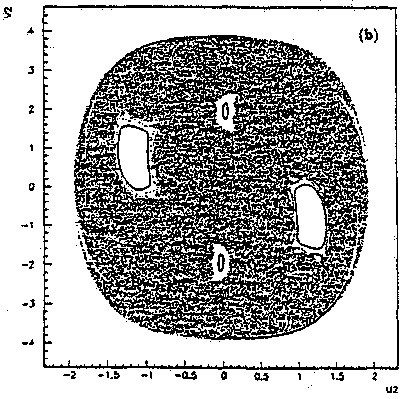
\includegraphics[height=0.45\textheight]{ponicare-sections-e_30}

    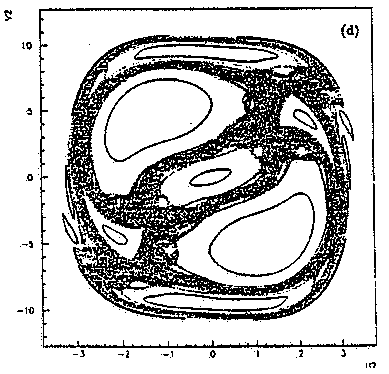
\includegraphics[height=0.45\textheight]{ponicare-sections-e_240}
  \end{column}
  \begin{column}{0.15\textwidth}
    \small \centering \(E = 30A\) \\
    \vspace{3cm}
    \(E = 240A\)
  \end{column}
  \begin{column}{0.35\textwidth}
    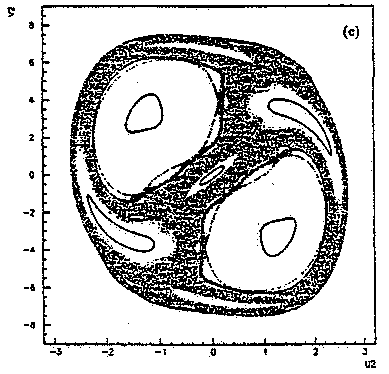
\includegraphics[height=0.45\textheight]{ponicare-sections-e_120}

    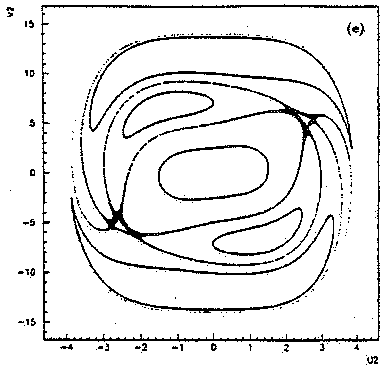
\includegraphics[height=0.45\textheight]{ponicare-sections-e_400}
  \end{column}
  \begin{column}{0.15\textwidth}
    \small \(E = 120A\) \\
    \vspace{3cm}
    \(E = 400A\)
  \end{column}
  \end{columns}
\end{frame}

%%%%%%%%%%%%%%%%%%%% slide 20 %%%%%%%%%%%%%%%%%%%%%%%%%%%%%%%%%%%%

\begin{frame}
  \begin{columns}[c]
  \begin{column}{0.35\textwidth}
    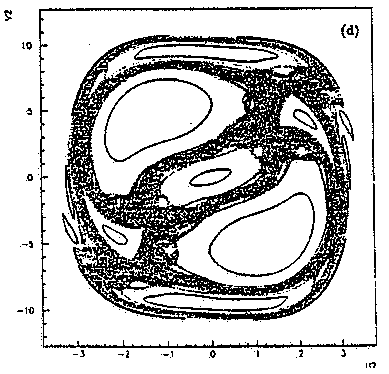
\includegraphics[height=0.45\textheight]{ponicare-sections-e_240}

    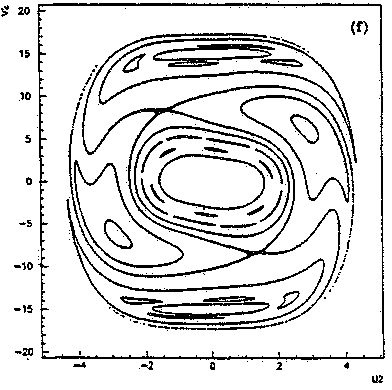
\includegraphics[height=0.45\textheight]{ponicare-sections-e_600}
  \end{column}
  \begin{column}{0.15\textwidth}
    \small \centering \(E = 240A\) \\
    \vspace{3cm}
    \(E = 600A\)
  \end{column}
  \begin{column}{0.33\textwidth}
    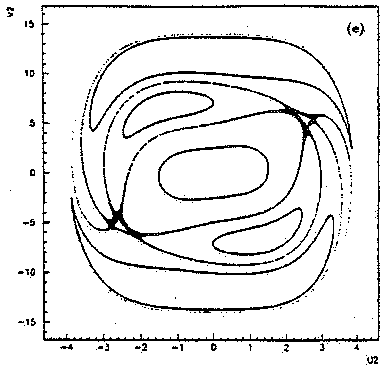
\includegraphics[height=0.45\textheight]{ponicare-sections-e_400}

    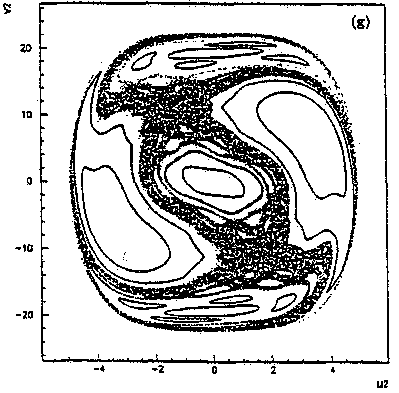
\includegraphics[height=0.45\textheight]{ponicare-sections-e_1000}
  \end{column}
  \begin{column}{0.17\textwidth}
    \small \centering \(E = 400A\) \\
    \vspace{3cm}
    \(E = 1000A\)
  \end{column}
  \end{columns}
\end{frame}

%%%%%%%%%%%%%%%%%%%% slide 21 %%%%%%%%%%%%%%%%%%%%%%%%%%%%%%%%%%%%

\begin{frame}
  \begin{itemize}
    \item The global phase space structure is reflected in the plot of
    \(\alpha \) as a function of \(\Delta E\)
  \end{itemize}
  \begin{columns}[c]
  \begin{column}{0.5\textwidth}
    \includegraphics[width=\textwidth]{{"alpha_e_B[0.55, 0.6, 0.63]"_N[260]}.pdf}  % chktex 36
  \end{column}
  \begin{column}{0.5\textwidth}
    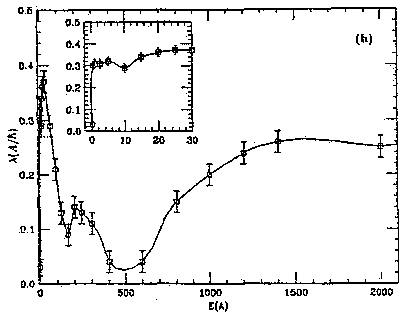
\includegraphics[width=\textwidth]{liapunov}
  \end{column}
  \end{columns}
\end{frame}

%%%%%%%%%%%%%%%%%%%% slide 22 %%%%%%%%%%%%%%%%%%%%%%%%%%%%%%%%%%%%

\begin{frame}
  \begin{itemize}
    \item The nontrivial dependence of \(\alpha \) on the non-integrability
    parameter \(B\) for \(N=220, 240, 260\)
  \end{itemize}
  \includegraphics[width=0.9\textwidth]{"alpha_N[220, 240, 260]".pdf}  % chktex 36
\end{frame}

%%%%%%%%%%%%%%%%%%%% slide 23 %%%%%%%%%%%%%%%%%%%%%%%%%%%%%%%%%%%%

\begin{frame}
  \begin{itemize}
    \item The qualitative stability of the shape of \(\alpha(B)\) when
    considering \(N=260\) and different values for the energy interval
  \end{itemize}
  \begin{columns}[c]
  \begin{column}{0.5\textwidth}
    \includegraphics[width=\textwidth]{{alpha_N[260]_max_e_"[100.0, 120.0, 140.0]"}.pdf}  % chktex 36
  \end{column}
  \begin{column}{0.5\textwidth}
    \includegraphics[width=\textwidth]{{alpha_N[260]_max_e_"[140.0, 160.0, 0.0]"}.pdf}  % chktex 36
  \end{column}
  \end{columns}
\end{frame}

%%%%%%%%%%%%%%%%%%%% slide 24 %%%%%%%%%%%%%%%%%%%%%%%%%%%%%%%%%%%%

\begin{frame}
  \begin{itemize}
    \item The qualitative stability of the shape of \(\alpha(B)\) when
    considering \(N=220, 240, 260\) and different values for the energy interval
  \end{itemize}
  \begin{columns}[c]
  \begin{column}{0.5\textwidth}
    \includegraphics[width=\textwidth]{{"alpha_N[220, 240, 260]"_max_e_[100.0]}.pdf}  % chktex 36
  \end{column}
  \begin{column}{0.5\textwidth}
    \includegraphics[width=\textwidth]{{"alpha_N[220, 240, 260]"_max_e_[140.0]}.pdf}  % chktex 36
  \end{column}
  \end{columns}
\end{frame}

\section{Conclusions}

%%%%%%%%%%%%%%%%%%%% slide 25 %%%%%%%%%%%%%%%%%%%%%%%%%%%%%%%%%%%%

\begin{frame}{Conclusions}
  \begin{itemize}
    \item We emphasised a correlation between the global phase space
    structure of the classical system and its quantum corespondent.
    \item We proposed a description of the nearest neighbour distribution of
    our spectra through a \emph{superposition of Poisson and Wigner distributions}.
    \item A non-trivial dependence of the superposition coefficient on the
    non-integrability parameter was revealed.
    \item Through our analysis we showed a correlation between the tori volume
    in classical phase space and the deviation from the Wigner distribution
    in the quantum system.
  \end{itemize}
\end{frame}

\end{document}
